

\chapter{An adaptive implicit-midpoint-rule time-integrator}
\label{sec:adaptive-imr}


The implicit midpoint rule (IMR)is a well known time integration method\cite[??ds]{HairerWanner} with a number of favourable properties as discussed in Section~\ref{sec:fixed-step-implicit}.
It is also known as the midpoint method and the ??ds.

% It is an implicit Runge-Kutta method, but unlike most such methods it only requires a single fuction evaluation per time step (a ``one-leg-method''\cite[??ds]{Hairer..}), making it applicable in cases where multistep methods would typically be applied.

% It is A-stable, meaning that it has unconditional stability for the standard test ODE.

% It has no spurious modes, meaning that it does not incorrectly cause the damping out of oscillations in the solution (like TR but unlike BDF methods).

% If does not suffer from ``ringing'' errors--non-physical oscillations in the solution which can cause difficulties with large time steps \cite{silvester etc. stab-TR}.

% Additionally, for linear problems, it is equivalent to the trapezoid rule which has the lowest possible local trunction error in an A-stable method\cite{??ds}.
% For non-linear problems the local truncation error is more complex, but still small...

The implicit midpoint rule also beneficial ``geometric integration'' properties when applied the Landau-Lifshitz-Gilbert equation, this is discussed in Section~\ref{sec:aimr-llg}.
It also has energy conservation properties when applied to the Navier-Stokes equations \cite{wind farms thesis}.


In this \secpaper{} we describe an efficient adaptive time step selection algorithm for the implicit midpoint rule. To our knowledge this is the first such algorithm.

\section{Fixed step implicit midpoint rule}
\label{sec:fixed-step-implicit}

Let $\yv(t)$ be a vector function, let $\yv_n$ denote an estimate to $\yv(t)$ at $t = t_n$.
Let $\dtn = t_{n+1} - t_n$ be the $n$th time step (or just ``step'').
Then given a system of equations of the form
\begin{equation}
  \yv'(t) = \fv(t, \yv(t)),
  \label{eq:43}
\end{equation}
the implicit midpoint rule (IMR) is
\begin{equation}
    \yv_{n+1} = \yv_n + \dtn \fv(\frac{t_{n+1} + t_n}{2}, \frac{\yv_n + \yv_{n+1}}{2}).
    \notag
\end{equation}
We write
\begin{equation}
  \begin{aligned}
    \frac{t_{n+1} + t_n}{2} &= \thf, \\
    \frac{\yv_{n+1} + \yv_n}{2} &= \yvm,
  \end{aligned}
\end{equation}
for readability, giving
\begin{equation}
  \yv_{n+1} = \yv_n + \dtn \fv(\thf, \yvm).
  \label{eq:basic-midpoint}
\end{equation}

Note that unlike multistep methods, such as the second order backwards difference (BDF2), this is valid for both constant and variable step sizes because there is no dependence on previous steps.

Next we discuss some properties of IMR as applied to ODEs and compare them to some other widely used time integration methods.
The other methods we compare with are BDF2 and the trapezoid rule (TR), because they have very similar stability, accuracy and computational cost to IMR.
All three are sufficiently stable and accurate for general use in PDE applications.

\subsection{Local truncation error and order}
\label{sec:deriv-local-trunc}

The local truncation error (LTE) of a time integration scheme is the error due a single integration step.
It can be calculated by substituting $\yv_n = \yv(t_n)$ into the approximation for the next time-step then subtracting the result from the exact solution at the next time-step, $\yv(t_{n+1})$.

Using this definition the local truncation error of IMR is
\begin{align}
  \lte^\imr &=  \yv(t_{n+1}) - \yv(t_n) - \dtn \fv\left( \thf, \frac{\yv(t_n) + \yv_{n+1}^\imr}{2} \right).
              \label{eq:trunc-start}
\end{align}

It is important to distinguish the local truncation error from the global (temporal) error
\begin{equation}
  \label{eq:global-temporal-error}
  \begin{aligned}
    E_n^\imr &= \yv(t_{n+1}) - \yv_{n+1}^\imr, \\
    &=  \yv(t_{n+1}) - \yv_n^\imr - \dtn \fv\bigb{ \thf, \frac{\yv_n^\imr + \yv_{n+1}^\imr}{2} }
  \end{aligned}
\end{equation}


The difference is that the global error includes any error accumulated over previous time steps.

We now partially calculate the IMR local truncation error.
We choose to Taylor expand everything about the midpoint, $\thf$, because it reduces the complexity of the result (and allows easier calculations).\footnote{If instead chose to expand about $t_n$ there would be an additional term in $\yv_n''$ in equation~\eqref{eq:trunc-mid}.}
Assuming that $\yv(t)$ is ``sufficiently smooth'' to have a Taylor series expansion, its Taylor series expansion at $t_{n+1}$ about $\thf$ is given by
\begin{equation}
  \yv(t_{n+1}) = \yv(\thf + \frac{\dtn}{2}) = \yvhf + \frac{\dtn}{2} \yvhf['] + \frac{\dtn^2}{8} \yvhf[''] + \frac{\dtn^3}{48} \yvhf['''] \porder{\dtn^4}.
  \label{eq:taylornp1}
\end{equation}
%% It is well known that the local truncation error of the midpoint rule is $\order{\dtn^3}$ (\ie it is second order)\cite{??ds}, so we can safely ignore $\order{\dtn^4}$ terms.
Similarly the expansion at $t_n$ is
\begin{equation}
  \yv(t_n) = \yv(\thf - \frac{\dtn}{2}) = \yvhf - \frac{\dtn}{2} \yvhf['] + \frac{\dtn^2}{8} \yvhf[''] - \frac{\dtn^3}{48} \yvhf['''] \porder{\dtn^4}.
  \label{eq:taylorn}
\end{equation}

Substituting equations~\eqref{eq:taylornp1} and \eqref{eq:taylorn} into equation~\eqref{eq:trunc-start} gives
\begin{equation}
  \lte^\imr = \yv(t_{n+1}) - \yv_{n+1}^\imr
  = \frac{\dtn^3}{24} \yvhf[''']  + \dtn  \left[ \yvhf[']
    - \fv\left( \thf, \frac{\yv(t_n) + \yv_{n+1}}{2} \right) \right]  \porder{\dtn^4}.
  \label{eq:trunc-mid}
\end{equation}

There are two parts to this error: the first term (with $\yv'''_n$) is fairly standard in second order multistep time integrators.
However the second term is more complex, applying a Taylor expansion approach here would result in a Jacobian-like matrix of derivatives of $\fv$ with respect to $\yv$.
Hence we avoid expanding it further.
See Section~\ref{sec:full-imr-lte-calculation} for details of the rest of the Taylor expansion, which also proves that IMR is indeed a second order method.

The TR\cite[pg. 261]{Gresho-Sani} and BDF2\cite[pg. 715]{Gresho-Sani} methods are also second order, their local truncation errors are simpler:
\begin{equation}
  \label{eq:tr-lte}
  \lte^\tr = \yv_{n+1} - \yv(t_{n+1}) = -\frac{\dtn^3 \yv_n'''}{12}
  + \order{\dtn^4},
\end{equation}

\begin{equation}
  \label{eq:bdf2-lte}
  \lte^\bdf = \yv_{n+1} - \yv(t_{n+1}) = \frac{(\dtn + \dtx{n-1})^2}{\dtn(2\dtn + \dtx{n-1})}
  \frac{\dtn^3 \yv_n'''}{6}
  + \order{\dtn^4}.
\end{equation}


\subsection{A-stability}

A-stablility (the A does not stand for anything, it is just ``A'') is the property that a method is stable when used to integrate equation ??ds for all $\lambda$ with $\real{\lambda} \leq 0$. 
When $\real{\lambda} \geq 0$ the ODE itself is unstable and so stability is not expected in general.
A-stabilitiy is a reasonably good way to classify the suitability of a time integrator for solving stiff ODEs (such as those that often emerge from a semi-discretisation of a PDE).

All three of the methods discussed are A-stable.
Explicit methods are not A-stable ??ds check? \cite{??ds}, which is the main reason this thesis focuses on implicit methods.

The maximum order of an A-stable multistep method is 2 \cite[??ds]{HairerNorsettWanner}.



\subsection{L-stability}
\label{sec:imr-l-stability}


\subsection{Order reduction}

It is known that certain implicit Runge-Kutta methods\cite[pg. 156]{Atkinson1994} are susceptible to reduced accuracy when used to solve extremely stiff problems.
In the case of the implicit midpoint rule this is represented in the second term of the full LTE expression~\eqref{eq:trunc-final}: if the eigenvalues of $\dfdyhf$ are large then the error will be much larger than expected.

This effect should be automatically detected and adjusted for by an error estimator.

For comparison: TR and the BDF methods do not suffer from order reduction\cite[pg. 159]{Atkinson1994} (\ie they have no error term related to an error in $\yv$ used in $f$ because all evaluations are at integer time points).

% The IMR and the BDF1 methods are B-convergent, TR is not B-convergent, the BDF2 method does not fit into the framework used to analyse such methods\cite[pg. 231]{HairerNorsettWanner}\footnote{In this book IMR is refered to as the second order Gauss method, BDF1 is Radau IIA, TR is Lobatto IIIA \cite[pg. 72-76]{HairerNorsettWanner}.}.



\section{Construction of an LTE estimate}

\subsection{Error estimation approaches}
\label{sec:two-integrator-error}

Most truncation error estimators for implicit integrators (e.g. trapezoid rule, BDF2) use a Milne-device based method.\cite[pgs 707-716]{Gresho-Sani}
This means that they compute an additional explicit estimate of $y_{n+1}$ using the same input values/derivatives as the implicit method and to the same order of accuracy.
They then use algebraic rearrangements of the two LTE expressions to calculate an approximation of the LTE (typically to one order of accuracy better than the original calculations).
However due to the complexity of the local truncation error of the implicit midpoint rule there are some difficulties with this approach.
In particular the midpoint rule's LTE has a term giving the error due to the approximation $\yvm \sim \yvhf$.
This term cannot appear in the LTE expression for any time integrator that does not use the midpoint approximation (\ie any other useful integrator) and so this term of the error cannot be easily approximated using a Milne-device-like method.

An alternative approach, commonly used in Runge-Kutta time integrators, is to repeat the calculation at a higher accuracy and compare the two answers directly obtain an LTE estimate.
However of the derivative function ($f$ in equation~\eqref{eq:43}) are expensive,  and the calculation of a single step of a high order Runge-Kutta method requires a number of function evaluations.
Hence such approaches usually rely on pairs of Runge-Kutta methods which share most of their derivative evaluation points but have different orders of accuracy.
One example of this technique is the Dormand–Prince pair (order 4/5), as used in MATLAB's \texttt{ode45} function.
Unfortunately IMR uses a single derivative function evaluation at the optimal point in the time step to cause cancellation of higher order terms.
Hence there is no way to reuse this evaluation in a higher order method without at least two additional evaluations due to the loss of error cancellations that would be caused by adding a single additional evaluation.

Instead we use a little known explicit version of the third order backwards difference method (eBDF3) as the higher order integrator.
This requires only 3 history values and a single (explicit) derivative function evaluationin order to compute a 3rd order accurate step.
With this approach our estimate for the local truncation error is simply
\begin{equation}
  \label{eq:aimr-lte-est}
  \lte = \yv_{n+1}^{eBDF3} - \yv_{n+1}^\imr + \order{\dtn^4}.
\end{equation}
The eBDF3 method is not commonly known because it is unstable when used for more than a single step.
However for our purposes we only ever need a single step of the method since the IMR history values are always available, hence stability analysis is irrelevant.
This method could also be thought of (like most time integration methods) as a polynomial extrapolation of the solution which also fits the derivative at time $t_n$.

Alternatively a 3rd order Adams-Bashforth scheme (AB3) could be used, this requires three previous derivative values instead of $y$ values, which makes the initialisation of the scheme a little more complex and expensive. 
Additionally the calculation of coefficients for the variable step Adams-Bashforth schemes is more complex \cite[pg. 400]{HairerNorsettWanner}.
In contrast to eBDF2, AB3 is stable which may simplify testing.


\subsection{The variable step explicit backwards difference 3 method}

% backwards version:
% \begin{equation}
%   \begin{aligned}
%     \bdiff^0 f_n &= f_n, \\
%     \bdiff^{j+1} f_n &= \bdiff^{j} f_n - \bdiff^{j} f_{n-1}, \\
%     q(t) &= q(t_n + sh), \\ 
%     &= f(t_n) + s \bdiff f(t_n) + \frac{s(s+1)}{2} \bdiff^2 f(t_n) + \cdots \frac{s(s+1)\cdots(s+n-1)}{n!}\bdiff^n f(t_n), \\
%     &= \sum_{j=1}^{n} (-1)^j \begin{pmatrix} -s\\ j \\ \end{pmatrix}
%     \bdiff^j f(t_n).
%   \end{aligned}
% \end{equation}

The explicit bdf methods are explicit time integration methods derived using the same techniques as the usual implicit BDF methods.
The idea is to write down a divided difference representation of an interpolating polynomial, $q(t)$, through the points $y_i$, $i=n-k+1, \ldots, n+1$ (backward differences can be used for constant time steps, hence the name).
The derivative of the polynomial is then equated to the derivative $y'(t, y) = f(t, y)$ given as the ODE definition\cite[pg. 400]{HairerNorsettWanner}.
Equating the derivative at time $t_{n+1}$ gives the familiar implicit BDF methods.
If we instead equate the derivative at a previous time we obtain the explicit BDF methods \cite[pg. 364]{HairerNorsettWanner}.

The Newton divided differences are defined recursively by
\begin{equation}
  \label{eqn:divided-diff}
  \begin{aligned}
    y[t_{n+1}] &= y_{n+1}, \\
    y[t_{n+1}, t_n] &= \frac{y[t_{n+1}] - y[t_n]}{t_{n+1} - t_n}, \\
    y[t_{n+1}, t_n, t_{n-1}] &= \frac{y[t_{n+1}, t_n] - y[t_n, t_{n-1}]}{t_{n+1} - t_{n-1}}, \\
    \vdots
  \end{aligned}
\end{equation} 
The Lagrange interpolation polynomials can be expressed using these divided differences \cite[pg. 124]{BurdenFaires}, \cite[pg. 400]{HairerNorsettWanner} as
\begin{equation}
  \label{eqn:divided-diff-intp}
  \begin{aligned}
    p_k(t) &= y_{n+1} + \sum_{j=1}^k y[t_{n+1}, \ldots, t_{n+1-j}] \prod_{i=0}^{j-1} (t - t_{n+1-i}), \\
    &= y_{n+1} + y[t_{n+1}, t_n](t - t_{n+1}) + y[t_{n+1}, t_n, t_{n-1}](t - t_{n+1})(t - t_n) \\
    &\quad + y[t_{n+1}, t_n, t_{n-1}, t_{n-2}](t - t_{n+1})(t - t_n)(t - t_{n-1}) + \ldots \\
    &\quad + y[t_{n+1}, \ldots, t_{n+1-k}](t-t_{n+1})\cdots(t-t_{n-k}).
  \end{aligned}
\end{equation}

Differentiating with respect to $t$ gives (divided differences are constants, product term is handled with the chain rule)
\begin{equation}
  \begin{aligned}
    p_k'(t) &= y[t_{n+1}, t_n] + y[t_{n+1}, t_n, t_{n-1}]\bigb{(t - t_n) + (t - t_{n+1})} \\
    &\quad + y[t_{n+1}, t_n, t_{n-1}, t_{n-2}]\bigb{(t - t_n)(t - t_{n-1}) + (t - t_{n+1})(t - t_{n-1}) + (t - t_{n+1})(t - t_n)} \\
    &\quad + \ldots \\
    &\quad + y[t_{n+1}, \ldots, t_{n+1-k}]\bigb{(t-t_{n})\cdots(t-t_{n-k}) + \ldots + (t-t_{n+1})\cdots(t-t_{n-k+1})}, \\
    &= \sum_{j=1}^k y[t_{n+1}, \ldots, t_{n+1-j}] \sum_{l=0}^{j-1} \prod_{i=0, i \neq l}^{j-1} (t - t_{n+1-i}).
  \end{aligned}
\end{equation} 

Equating the derivative at time $t_n$ results in
\begin{equation}
  \begin{aligned}
    f(t_n, y_n) &= \sum_{j=1}^k y[t_{n+1}, \ldots, t_{n+1-j}] \sum_{l=0}^{j-1} \prod_{i=0, i \neq l}^{j-1} (t_n - t_{n+1-i}).
  \end{aligned}
\end{equation} 
This can be greatly simplified by noticing that the product $ \prod_{i=0, i \neq l}^{j-1} (t_n - t_{n+1-i})$ is zero whenever it contains $i=1$, \ie whenever $j \geq 2$ and $l \neq 1$.
However when $j=1$ the only terms in the sum of products are $l=0$ and $i=0$, so we only need to consider the case of $l=1$.
This gives
\begin{equation}
  \begin{aligned}
    f(t_n, y_n) &= \sum_{j=1}^k y[t_{n+1}, \ldots, t_{n+1-j}] \prod_{i=0, i \neq 1}^{j-1} (t_n - t_{n+1-i}), \\
    &= y[t_{n+1}, t_n] + \sum_{j=2}^k y[t_{n+1}, \ldots, t_{n+1-j}] \prod_{i=0, i \neq 1}^{j-1} (t_n - t_{n+1-i}), \\
    &= y[t_{n+1}, t_n] -\dtn \sum_{j=2}^k y[t_{n+1}, \ldots, t_{n+1-j}] \prod_{i=2}^{j-1} (t_n - t_{n+1-i}). \\
  \end{aligned}
\end{equation}

For $k=1$ we get
\begin{equation}
  \begin{aligned}
    f(t_n, y_n) &= y[t_{n+1}, t_n], \\
    &= \frac{y_{n+1} - y_n}{\dtn}, \\
    y_{n+1} &= y_n + \dtn f(t_n, y_n), \\
  \end{aligned}
\end{equation} 
which is forward Euler.

For $k=2$ we have
\begin{equation}
  \begin{aligned}
    f(t_n, y_n) &= y[t_{n+1}, t_n] - \dtn y[t_{n+1}, t_n, t_{n-1}] , \\
    &=  \frac{y_{n+1} - y_n}{\dtn} 
    - \frac{\dtn}{\dtn + \dtx{n-1}} \bigb{ \frac{y_{n+1} - y_n}{\dtn} - \frac{y_n - y_{n-1}}{\dtx{n-1}}}.
  \end{aligned}
\end{equation}
After some algebra this gives
\begin{equation}
  \label{eq:emr-derivation-rearranged}
  y_{n+1} = y_n + \bigb{1 + \frac{\dtn}{\dtx{n-1}}}\dtn f(t_n, y_n)
    - \frac{\dtn^2}{\dtx{n-1}^2}(y_n - y_{n-1}),
\end{equation}
which is the variable step equivalent of the leapfrog method (explicit midpoint rule) \cite[pg. 715]{GreshoSani}.

For larger values of $k$ the messyness of the algebra grows explosively.
Unfortunately we are interested in the third order method, so:
\begin{equation}
  \begin{aligned}
    f(t_n, y_n) &= y[t_{n+1}, t_n] - \dtn y[t_{n+1}, t_n, t_{n-1}] -\dtn y[t_{n+1}, t_n, t_{n-1}, t_{n-2}], \\
    &=  \frac{y_{n+1} - y_n}{\dtn} 
    - \frac{\dtn}{\dtn + \dtx{n-1}} \bigb{ \frac{y_{n+1} - y_n}{\dtn} - \frac{y_n - y_{n-1}}{\dtx{n-1}}} \\
    &\quad - \frac{\dtn}{\dtn + \dtx{n-1} + \dtx{n-2}}
         \bigs{
           \frac{\frac{y_{n+1} - y_n}{\dtn} - \frac{y_n - y_{n-1}}{\dtx{n-1}}}
                {\dtn +\dtx{n-1}}
           -
           \frac{\frac{y_{n} - y_{n-1}}{\dtn} - \frac{y_{n-1} - y_{n-2}}{\dtx{n-1}}}
                {\dtx{n-1} +\dtx{n-2}}
         }.
  \end{aligned}
\end{equation}
Doing this by hand is complex and error prone so a script was written to carry out algebraic rearrangement into coefficient form using the \texttt{python} programming language with the \texttt{sympy} library\cite{sympy}.
The output is \texttt{c++} source code for the coefficient vector (to avoid translation errors).
The resulting method (machine translated from the source code\cite[src/generic/explicit_timesteppers.cc:EBDF3::set_weights]{oomph-lib-source}) is
\begin{equation}
  \label{eqn:ebdf-coeffs}
  \begin{aligned}
    a y_{n+1} &= b f(t_n, y_n) + c_n y_n + c_{n-1} y_{n-1} + c_{n-2} y_{n-2}, \\
    a &= \dtx{n-1}^4 \dtx{n-2}  + \dtx{n-1}^3 \dtx{n-2}^2  
    + \dtx{n-1}^2 \dtx{n-2}^3 , \\
    b &= -(-\dtn^3 \dtx{n-1}^2 \dtx{n-2}  - \dtn^3 \dtx{n-1} \dtx{n-2}^2  
    - \dtn^2 \dtx{n-1}^3 \dtx{n-2}  
    - \dtn^2 \dtx{n-1}^2 \dtx{n-2}^2  \\
     & \quad - \dtn^2 \dtx{n-1} \dtx{n-2}^3  - \dtn \dtx{n-1}^4 \dtx{n-2}  
     - 2\dtn \dtx{n-1}^3 \dtx{n-2}^2  
     - \dtn \dtx{n-1}^2 \dtx{n-2}^3), \\ 
    c_n &= -(\dtn^3 \dtx{n-1} \dtx{n-2}  + \dtn^3 \dtx{n-2}^2  
    + \dtn^2 \dtx{n-1}^2 \dtx{n-2}  
    + \dtn^2 \dtx{n-1} \dtx{n-2}^2  + \dtn^2 \dtx{n-2}^3 \\
    &\quad - \dtx{n-1}^4 \dtx{n-2}  - \dtx{n-1}^3 \dtx{n-2}^2  
    - \dtx{n-1}^2 \dtx{n-2}^3 ), \\
    c_{n-1} & = -(-\dtn^3 \dtx{n-1}^2  - \dtn^3 \dtx{n-1} \dtx{n-2}  
    - \dtn^3 \dtx{n-2}^2  - \dtn^2 \dtx{n-1}^3  
    - \dtn^2 \dtx{n-1}^2 \dtx{n-2} \\
    &\quad - \dtn^2 \dtx{n-1} \dtx{n-2}^2  
    - \dtn^2 \dtx{n-2}^3 ), \\
    c_{n-2} &= -(\dtn^3 \dtx{n-1}^2  + \dtn^2 \dtx{n-1}^3 ).
  \end{aligned}
\end{equation}

??ds wrong, doesn't match up! Make the script emit latex?
Include code generation script in oomph-lib?

For constant time steps the result is much simpler:
\begin{equation}
  \begin{aligned}
    a &= 1/3, \\
    b &= \dtn,\\ 
    c_n &= -1/2,\\
    c_{n-1} & = 1,\\
    c_{n-2} &= -1/6.
  \end{aligned}
\end{equation} 
This matches with the result in \cite[pg. 364]{HairerNorsettWanner}.

It should be noted that as a time integrator the eBDF3 scheme is completely unstable.
However the way it is used here means that this does not matter--only single steps of eBDF3 are ever taken.
Subsequent steps are not based on previous eBDF3 outputs but instead on the outputs of the (very stable) IMR.

It should also be noted that the calculation of the coefficients in equation~\eqref{eqn:ebdf-coeffs} could be comparatively expensive if the number of y-values was small ($\sim \order{100}$ operations assuming no compiler optimisation of the multiplications).
However when used in finite-element or finite-difference calculations the number of values is at least tens of thousands, so the cost of equation~\eqref{eqn:ebdf-coeffs} is trivial by comparision with, for example, the calculation of $f(t_n, \yv_n)$.


\subsubsection{Implicit BDF derivations}
??ds don't really need this but helpful for comparisions, appendix?

Equating the derivative at time $t_{n+1}$ results in
\begin{equation}
  \begin{aligned}
    f(t_{n+1}, y_{n+1}) &= \sum_{j=1}^k y[t_{n+1}, \ldots, t_{n+1-j}] \sum_{l=0}^{j-1} \prod_{i=0, i \neq l}^{j-1} (t_{n+1} - t_{n+1-i}).
  \end{aligned}
\end{equation} 
This can be greatly simplified by noticing that the product $ \prod_{i=0, i \neq l}^{j-1} (t_{n+1} - t_{n+1-i})$ is zero whenever it contains $i=0$, \ie all terms in the sum with $l \neq 0$.
This gives
\begin{equation}
  \begin{aligned}
    f(t_{n+1}, y_{n+1}) &= \sum_{j=1}^k y[t_{n+1}, \ldots, t_{n+1-j}] \prod_{i=0, i \neq 0}^{j-1} (t_{n+1} - t_{n+1-i}), \\
    &=  y[t_{n+1}, t_n] + \sum_{j=2}^k y[t_{n+1}, \ldots, t_{n+1-j}] \prod_{i=1}^{j-1} (t_{n+1} - t_{n+1-i}). \\
  \end{aligned}
\end{equation}

For $k=1$ we get
\begin{equation}
  \begin{aligned}
    f(t_{n+1}, y_{n+1}) &= \frac{y_{n+1} - y_n}{\dtn}, \\
    y_{n+1} &= y_n + \dtn f(t_{n+1}, y_{n+1}),
  \end{aligned}
\end{equation}
which is backward Euler as expected.

For $k=2$
\begin{equation}
  \label{eqn:bdf2-derivation}
  \begin{aligned}
    f(t_{n+1}, y_{n+1}) &= \frac{y_{n+1} - y_n}{\dtn} +  y[t_{n+1}, t_{n}, t_{n-1}](t_{n+1} - t_n), \\
    &= \frac{y_{n+1} - y_n}{\dtn} +  \frac{\dtn}{\dtx{n+1} + \dtn} \bigb{\frac{y_{n+1} - y_n}{\dtn} - \frac{y_n - y_{n-1}}{\dtx{n-1}}}. \\
  \end{aligned}
\end{equation}
After some algebra this is
\begin{equation}
  \label{eqn:bdf2-derivation-rearranged}
  \begin{aligned}
    \frac{y_{n+1} - y_n}{\dtn} = \frac{\dtn}{2\dtn + \dtx{n-1}} \frac{y_n - y_{n-1}}{\dtx{n-1}} 
    + \frac{\dtn + \dtx{n-1}}{2\dtn + \dtx{n-1}} f(t_{n+1}, y_{n+1}).
  \end{aligned}
\end{equation}
as expected for BDF2 \cite[pg. 715]{GreshoSani}.


\subsection{Computing the size of the next step}

We use a standard method \cite[pg.268]{Gresho-Sani} for computing the next step size from the local truncation error and a target local truncation error $\toltt$
\begin{equation}
\dtx{n+1} = \dtn \left( \frac{\toltt}{\lte}  \right) ^{\frac{1}{\texttt{order}+1}}.
\end{equation}
For implicit midpoint rule this is
\begin{equation}
  \dtx{n+1} = a \dtn \bigb{ \frac{\toltt}{\abs{\yv_{n+1}^{eBDF3} - \yv_{n+1}^\imr}} }^{\frac{1}{3}}.
\end{equation}

If the ratio of step size to desired step size is too low, \ie if the step just taken was much too large to attain the desired accuracy then we reduce the step size by a factor of 2 and repeat the step.

Actually we (should) include a slight safety factor, $a \sim 1/2$ to reduce the number of step rejections:
??ds but actually oomph-lib doesn't...
??ds check what CVODE, Iserles use as safety factor


Additionally we impose a limitation on the maximum step size scaling to help improve stability ??ds does this actually do anything?


??ds this is still flakey, test things? Use reltol? Ask Matthias?

A final modification is to include limitations on the step size that prevent issues with numerical accuracy.
We assume that the equations being modelled are non-dimensionalised so that the initial Newton residual (see Section~\ref{sec:newt-raph}) is $\sim \order{\dtn}$ (The initial guess is the value at the previous step, the change in the solution value in one step should be of size somewhere around $\dtn$).
In this case the minimum time step we can take is approximately the Newton tolerance (otherwise the Newton method will converge ``early'' because the residual is small to begin with).
Similarly the maximum time step we can take is $\sim \order{\frac{\texttt{newtontol}}{10^{-16}} = 10^{8}}$ before the Newton method will have difficulty converging due to numerical errors.


Note that some alternative strategies try to minimise the number of modifications to the time step size \cite[chap. 6]{Iserles2009} \cite[Sec. 2.1]{cvode-manual}.
The motivation for this is the use of a modified Newton-Raphson method where the Jacobian is not recalculated at each Newton step.
In the case of ODE solvers this is extremely beneficial because the Jacobian is usually dense and direct solvers are used to solve it--by keeping the Jacobian constant the number of solves and Jacobian assemblys are greatly reduced.
The downside is a reduction in the convergence speed of the Newton method.
Keeping the step size constant for as long as possible is required here because modifications to the time step cause modifications to the Jacobian.
However for PDE solvers, and in particular for iterative PDE solvers there is little-to-no benefit in using this technique (the reduction in convergence speed is worse than the gain of not assembling/solving the sparse Jacobian\cite[pg. 128]{Iserles2009}.


\section{Numerical experiments}
\label{sec:aimr-testing}

In this Section we show the results of some initial testing of the adaptive IMR algorithm derived above on some simple ODE examples.
Numerical experiments with the LLG equation are detailed in Section~\ref{sec:aimr-llg}.


\subsection{Implementation}
\label{sec:aimr-implementation}

We compare the adaptive IMR developed above with two commonly used adaptive implicit time integrators:
\begin{itemize}
\item Standard adaptive trapezoid rule. 
  The error estimate is construted by comparison with a step of the explicit second order Adams method in combination with some calculations involving the local truncation errors of both methods (known as Milne's device) \cite[pg. 707]{GreshoSani}.
\item Adaptive BDF2, with the error estimate again constructed using Milne's device from the variable step leapfrog method (\ie explicit BDF2) \cite[pg. 715]{GreshoSani}.
\end{itemize}

All three methods are implemented within the \texttt{oomph-lib} framework.
To increase relevance to the general non-linear PDE case (such as the LLG equation) we use exactly the same methods for the solution of the ODEs as used for semi-discretised PDEs.
So we use the Newton-Raphson method with a finite-differenced Jacobian inverted by a linear solver.
One effect of this is that the ``numerical error'' as seen by the ODE solver is equivalent to the Newton tolerance.

Unless otherwise specified all examples in this section use a Newton tolerance of $\newtontol = 10^{-8}$, an initial time step of $\dtx{0} = 10^{-6}$ and an adaptive integrator tolerance of $\toltt = 10^{-4}$.
Any initial conditions required are calculated from the exact solutions.

In all cases the exact solution is visually indistinguishable from the approxmated solutions on the scale of the plots.

For each example:
??ds exact solution (combine with below?)
??ds step sizes plot - show bdf2, tr and imr?
??ds convergence plot - shrink eps
??ds plot lte est and y'''?


\subsection{Polynomial example}
\label{sec:imr-polynomial-example}

The first example used is an ode with a 2nd order polynomial as the exact solution.
\begin{equation}
  \label{eqn:imr-test-poly2}
  \begin{aligned}
    y(t) &= t^2 + 0.5, \\
    f(t,y) &= 2t, \\
    y(0) & = 0.5.
  \end{aligned}
\end{equation}
This should be integrated exactly by IMR, or any other second order method, since $\lte \propto y'''(t) \equiv 0$.
So the adaptivity should detect this and increase the time step at the maximum allowed rate.

The results of this experiment are shown in Figure~\ref{fig:imr-poly2-example}. 
As expected all three methods keep the error extremely small (below or around the Newton tolerance) even for extremely large time steps.
The step size increases rapidly for all methods, again as would be expected.
The computed solution does not look much like a polynomial because the distance between output points is so large (due to large time steps).

\begin{figure}[h!]
  \centering
  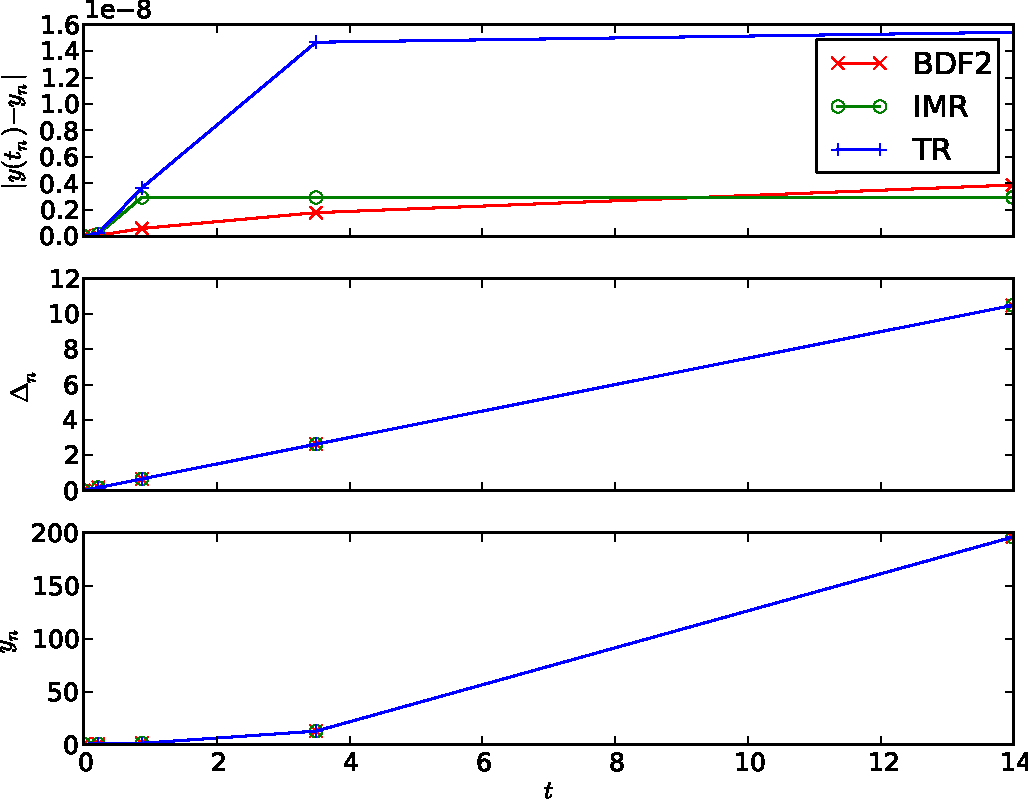
\includegraphics[width=1\textwidth]{images/poly2-errornormsvs-dtsvs-tracevaluesvstimes}
  \caption{Absolute error, time step size and computed solutions for the example ODE with exact solution $y(t) = at^2 + bt + c$.}
  \label{fig:imr-poly2-example}
\end{figure}


\subsection{Oscillatory, damped example}
\label{sec:oscill-damp-example}

The next test is an oscillatory function with damping
\begin{equation}
  \label{eqn:imr-test-osc-damp}
  \begin{aligned}
    y(t) &= e^{-\beta t} \sin(\omega t), \\
    f(t,y) &= - \beta e^{-\beta t} \sin(\omega t) + \omega e^{-\beta t} \cos(\omega t).  \end{aligned}
\end{equation} 
The adaptive algorithm should oscillate the step size in time with the oscillating truncation error ($\pd{}{t^3} \sin(t) = -\cos(t)$), while at the same time gradually increasing the step size as the solution damps to zero.

\begin{figure}[h!]
  \centering 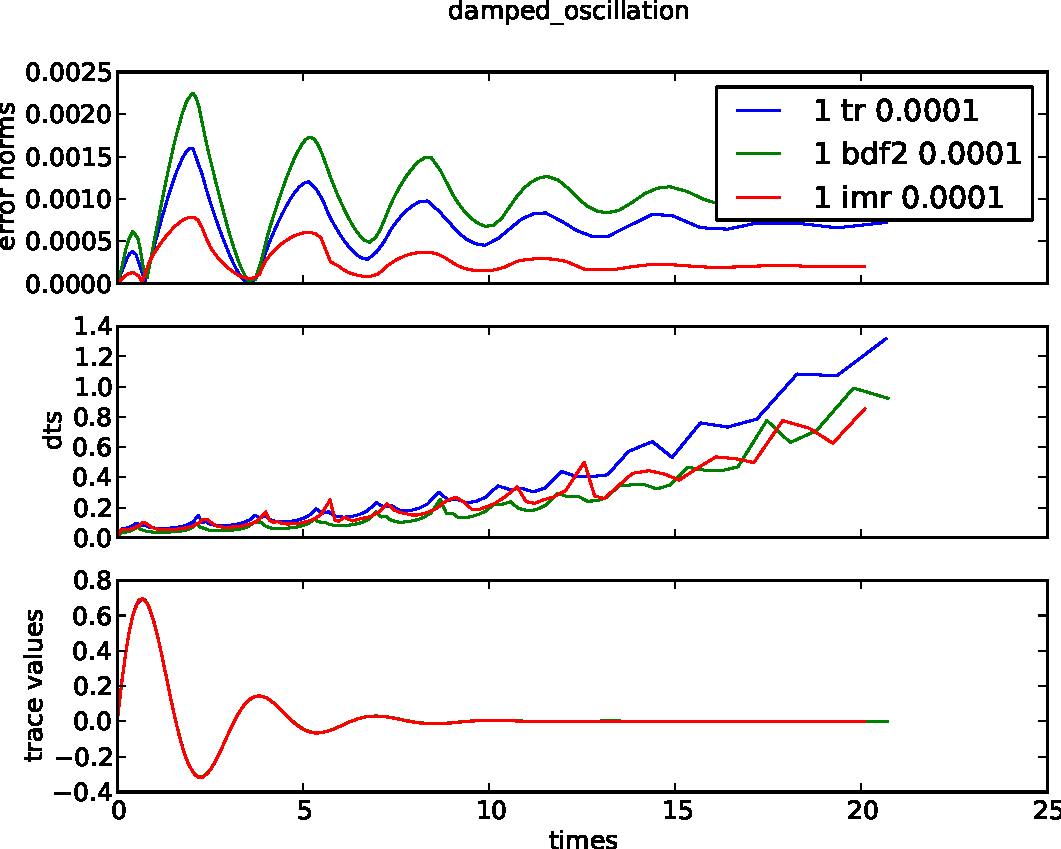
\includegraphics[width=1\textwidth]{images/damped_oscillation-errornormsvs-dtsvs-tracevaluesvstimes}
  \caption{Absolute error, time step size and computed solutions for the oscillatory, damped example ODE with exact solution $y(t) = e^{-\beta t} \sin(\omega t)$.}
  \label{fig:imr-osc-example}
\end{figure}

The ODE was solved with parameters $\omega = 2 \pi$ and $\beta = 0.5$, the results are shown in Figure~\ref{fig:imr-osc-example}.
All three methods have similar errors and time step sizes.
The IMR method choses slighly smaller steps than TR (which probably explains the slightly lower error magnitudes.
BDF2 has the worst errors as expected because its error coefficient is the largest.

Note that the plot shows the global (temporal) error, whereas the error estimates used for step size selection calculations are for the local error--the additional error introduced by a single step.
Hence the fact that the errors increase above the tolerance is not suprising.

Interestingly there is a slight lag on the time step response of the IMR method as time steps become larger.
This could be due to the fact that IMR uses data from three previous steps in its LTE estimate, whereas the others only use two previous steps.




\subsection{Stiff example}
\label{sec:imr-stiff-example}

Another test is the simple and commonly discussed stiff example function \cite{??ds Iserles?}
\begin{equation}
  \label{eqn:imr-test-stiff}
  \begin{aligned}
    f(t, \yv) &= \begin{pmatrix}
     -\lambda & 1 \\
      -0.1 & 0 \\
    \end{pmatrix}   \yv, \\
    % 
    \yv(t) &= 
    \begin{pmatrix} e^{-0.1t} \\ (\lambda - 0.1)e^{-\lambda t} \end{pmatrix}.
    %
    % \yv(0) &= \begin{pmatrix} 1  \\ \lambda - 0.1  \\ \end{pmatrix}.
  \end{aligned}
\end{equation} 
This example will demonstrate that the single step of the eBDF method does not suffer from stability issues even in cases of extreme stiffness.
The time steps should begin small but rapidly increase as the initial transient decays.

The results of the applying the three methods to problem~\eqref{eqn:imr-test-stiff} with $\lambda = -100$ (fairly stiff) are shown in Figure~\ref{fig:imr-stiff-example}.
The behaviour of the three time integrators is essentially the same, indicating that our adaptive IMR has no issues with stiffness.

\begin{figure}[h!]
  \centering
  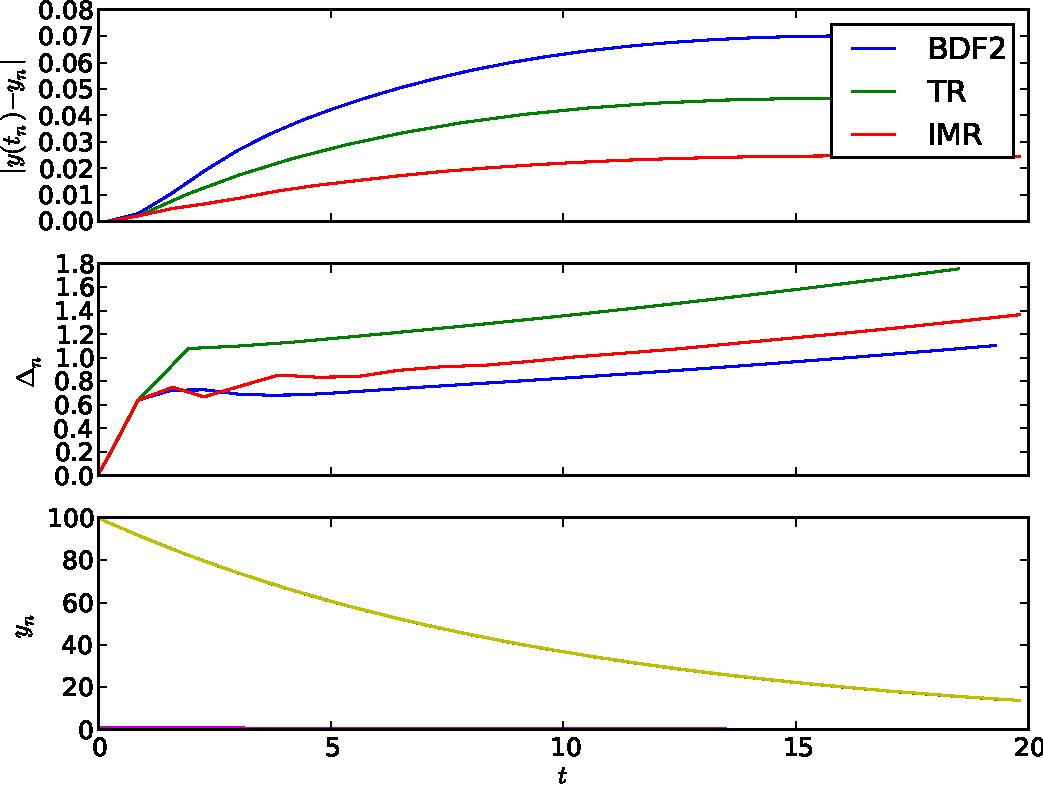
\includegraphics[width=1\textwidth]{images/stiff_test-errornormsvs-dtsvs-tracevaluesvstimes}
  \caption{Error $2$-norm, time step size and computed solutions for the stiff example ODE.}
  \label{fig:imr-stiff-example}
\end{figure}

??ds multiple stiffness parameter values?


\subsection{Order reduction example}
\label{sec:order-reduct-example}

As a final example we use a test ODE for order reduction/extreme stiffness\cite[pg. 156]{Atkinson2009}
\begin{equation}
  \label{eqn:imr-test-order-reduction}
  \begin{aligned}
    f(t, y) &= \lambda (y - g(t)) + g'(t), \\
    y(t) &= g(t), \\
  \end{aligned}
\end{equation}
for some function $g(t)$ and large negative parameter $\lambda$.

This causes an order reduction effect when solved using IMR because $\pd{f}{y} = \lambda$, and so when $\lambda$ is large the second term of the LTE expression~\eqref{eq:trunc-mid} becomes large.

We expect to see the adaptive IMR perform similarly to a first order adaptive implicit method which does not suffer from order reduction.
Both the adaptive IMR and the first order method should select much smaller time steps than TR and BDF2 in order to control the errors.
To test this we also run the experiment with an adaptive BDF1 (backwards Euler) method using Milne's method for adaptivity.

For the experiments we chose an oscillatory function, $g(t) = sin(t) + cos(t)$, because it highlights the differences well.
As in the previous example we choose $\lambda = 100$. 



\begin{figure}[h!]
  \centering  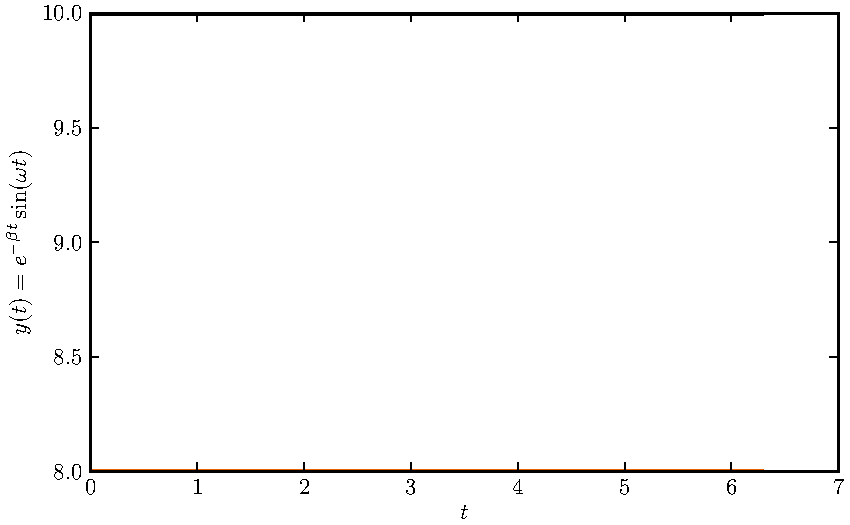
\includegraphics[width=1\textwidth]{images/order_reduction_test-errornormsvs-dtsvs-tracevaluesvstimes}
  \caption{Absolute error, time step size and computed solutions for the stiff order reduction example ODE given in equation~\eqref{eqn:imr-test-order-reduction}
.}
  \label{fig:imr-order-reduction-example}
\end{figure}

The results are shown in Figure~\ref{fig:imr-order-reduction-example}. 
??ds discussion


\subsection{General discussion}
\label{sec:aimr-general-discussion}

Figures~??ds compare mean error norms and step sizes of the adaptive midpoint scheme (with two interpolation points) for varying tolerances.
The IMR can be seen to have quadratic convergence by comparing with the $y=x^2$ line shown.
Additionally it can be seen that decreasing the tolerance smoothly decreases the mean error (by smoothly decreasing the mean step size).

In general more accurate than bdf2 due to lower error coeff (see Appendix??ds), similar error to tr.

\section{Additional Notes}

\subsection{Application to Implicit ODEs}
\label{sec:extens-impl-odes}

We sometimes wish to solve a system of equations where $\yv'(t)$ only given implicitly\footnote{This use of ``implicit'' is unrelated to the notion of implicitness in the time integration scheme.} (for example the Gilbert form of the Landau-Lifshitz-Gilbert equation), in this case equation~\eqref{eq:43} becomes
\begin{equation}
  \fv(t, \yv(t), \yv'(t)) = 0.
\end{equation}

We note that equation~\eqref{eq:basic-midpoint} can also be written in the from
\begin{equation}
  \yv'(\thf) = \frac{\yv_{n+1} - \yv_n}{\dtn} =  \fv(\thf, \frac{\yv_n + \yv_{n+1}}{2}).
\end{equation}
So the obvious equivalent for IMR is
\begin{equation}
  \fv(\thf, \frac{\yv_{n+1} + \yv_n}{2}, \frac{\yv_{n+1} - \yv_n}{\dtn}) = 0.
\end{equation}

However the adaptive scheme requires an additional function evaluation.
For implicitly defined functions this is expensive, so this adaptive method is not efficient for equations which can only be defined in such a way.





%%% Local Variables:
%%% mode: latex
%%% TeX-master: "./main"
%%% End:
